% These are the lecture notes for my CSCI360 course SPRING 2017
% at John Jay College of Criminal Justice.

% Feel free to edit these slides and use them for your own courses.
% HOWEVER DO NOT REMOVE THESE LINES!
% Email me at: awood [at] jjay.cuny.edu
% or at: awood [at] gradcenter.cuny.edu


\documentclass{beamer}

\usepackage{tikz}
\usetikzlibrary{calc}

\usepackage{forest}
\usepackage{verbatim}
\usepackage{color}


\setbeamertemplate{footline}[frame number]
\setbeamertemplate{navigation symbols}{} 

\newtheorem{thm}{Theorem}[section]
\newtheorem{lem}{Lemma}
\newtheorem{cl}{Claim}
\newtheorem{cor}{Corollary}[section]
\newtheorem{conj}{Conjecture}
\newtheorem{quest}{Question}
\newtheorem{defn}{Definition}[section]
\newtheorem{obs}{Observation}[section]
\newtheorem{exam}{Example}

\newcommand{\im}{\operatorname{im}}
\newcommand{\id}{\operatorname{id}}
\newcommand{\interior}{\operatorname{int}}
\newcommand{\bdry}{\operatorname{bdry}}
\newcommand{\<}{\langle}
\renewcommand{\>}{\rangle}
\newcommand{\Gab}{(G_\phi)^{ab}} 
\newcommand{\phibar}{\bar{\phi}}
\newcommand{\Z}{\mathbb{Z}}
\newcommand{\N}{\mathbb{N}}
\newcommand{\Q}{\mathbb{Q}}
\newcommand{\R}{\mathbb{R}}
\newcommand{\C}{\mathbb{C}}
\newcommand{\A}{\mathcal{A}}
\newcommand{\OO}{\mathcal{O}}
\newcommand{\UU}{\mathcal{U}}
\newcommand{\power}{2^{\{P_1, \cdots , P_n\}}}
\newcommand{\bp}{\begin{problem}}
\newcommand{\ep}{\end{problem}}
\newcommand{\ba}{\begin{answer}}
\newcommand{\ea}{\end{answer}}
\newcommand{\ds}{\displaystyle}
\newcommand{\ben}{\renewcommand{\theenumi}{\alph{enumi}}
\renewcommand{\labelenumi}{(\theenumi)}\begin{enumerate}}
\newcommand{\een}{\end{enumerate}}
\newcommand{\Hess}{\operatorname{Hessian}}
\newcommand{\Aut}{\mathrm{Aut}}
\newcommand{\Inn}{\mathrm{Inn}}
\newcommand{\Out}{\mathrm{Out}}
\newcommand{\End}{\mathrm{End}}


\mode<presentation>
{
%  \usetheme{default}
  \setbeamercovered{invisible}
}


\usepackage[english]{babel}
\usepackage[latin1]{inputenc}
\usepackage{times}
\usepackage[T1]{fontenc}
\usepackage{stmaryrd}

%\usetheme{default}
%\usetheme{AnnArbor}
%\usetheme{Antibes}
%\usetheme{Bergen}
%\usetheme{Berkeley}
%\usetheme{Berlin}
%\usetheme{Boadilla}
%\usetheme{CambridgeUS}
%\usetheme{Copenhagen}
%\usetheme{Darmstadt}
%\usetheme{Dresden}
%\usetheme{Frankfurt}
%\usetheme{Goettingen}
%\usetheme{Hannover}
%\usetheme{Ilmenau}
%\usetheme{JuanLesPins}
%\usetheme{Luebeck}
%\usetheme{Madrid}
%\usetheme{Malmoe}
%\usetheme{Marburg}
%\usetheme{Montpellier}
%\usetheme{PaloAlto}
%\usetheme{Pittsburgh}
%\usetheme{Rochester}
\usetheme{Singapore}
%\usetheme{Szeged}
%\usetheme{Warsaw}

%\usecolortheme{default}
%\usecolortheme{albatross}
\usecolortheme{beaver}
%\usecolortheme{beetle}
%\usecolortheme{crane}
%\usecolortheme{dolphin}
%\usecolortheme{dove} % grey, white, yellow
%\usecolortheme{fly} %grey, yellow
%\usecolortheme{lily} %white, yellow, blue
%\usecolortheme{orchid}
%\usecolortheme{rose}
%\usecolortheme{seagull}
%\usecolortheme{seahorse}
%\usecolortheme{whale}
%\usecolortheme{wolverine}

% Title page

\title[CSCI360]{The Enigma Machine and the Bombe: \\ Cryptology during WWII}

\author
{Lecture notes of Alexander Wood \\ CSCI 360 Cryptography and Cryptanalysis \\ \scriptsize \href{mailto:awood@jjay.cuny.edu}{awood@jjay.cuny.edu}}
\institute[JJay]{John Jay College of Criminal Justice}  

\date{}

\begin{document}

% Remove 'figure' text from figure captions 
\setbeamertemplate{caption}{\raggedright\insertcaption\par}

\begin{frame}
  \titlepage
\end{frame}


\section{Creation} 

\begin{frame}
\frametitle{The Enigma Machine}
\begin{columns}
\begin{column}{.5\textwidth}
The Enigma Machine was designed by the German engineer Arthur Scherbius. He began manufacturing the machine in 1923, shortly after which it was adopted and manufactured by the German navy, army, and air force. 
\end{column}
\begin{column}{.5\textwidth}
\begin{figure}
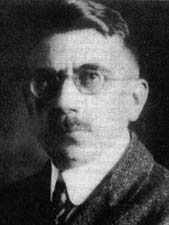
\includegraphics[scale=1]{IMG/scherbius.jpg}
\caption{\scriptsize Arthur Scherbius}
\end{figure}
\end{column}
\end{columns}
\end{frame}


\begin{frame}
\frametitle{Enigma Model A}
\begin{columns}
\begin{column}{.5\textwidth}
\begin{figure}
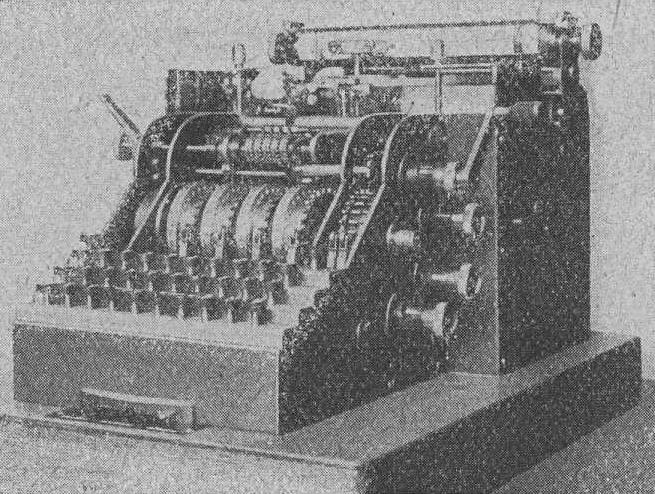
\includegraphics[scale=.3]{IMG/modelA.jpg}
\caption{\scriptsize from cryptomuseum.com}
\end{figure}
\end{column}

\begin{column}{.5\textwidth}
The first design of the Enigma machine, called Model A, weighed 50 kg and was similar in size to a cash register. \newline

``Enigma'' is German for ``riddle.''
\end{column}
\end{columns}
\end{frame}


\begin{frame}
\frametitle{Enigma Model B \& C}
\begin{columns}
\begin{column}{.5\textwidth}
\begin{figure}
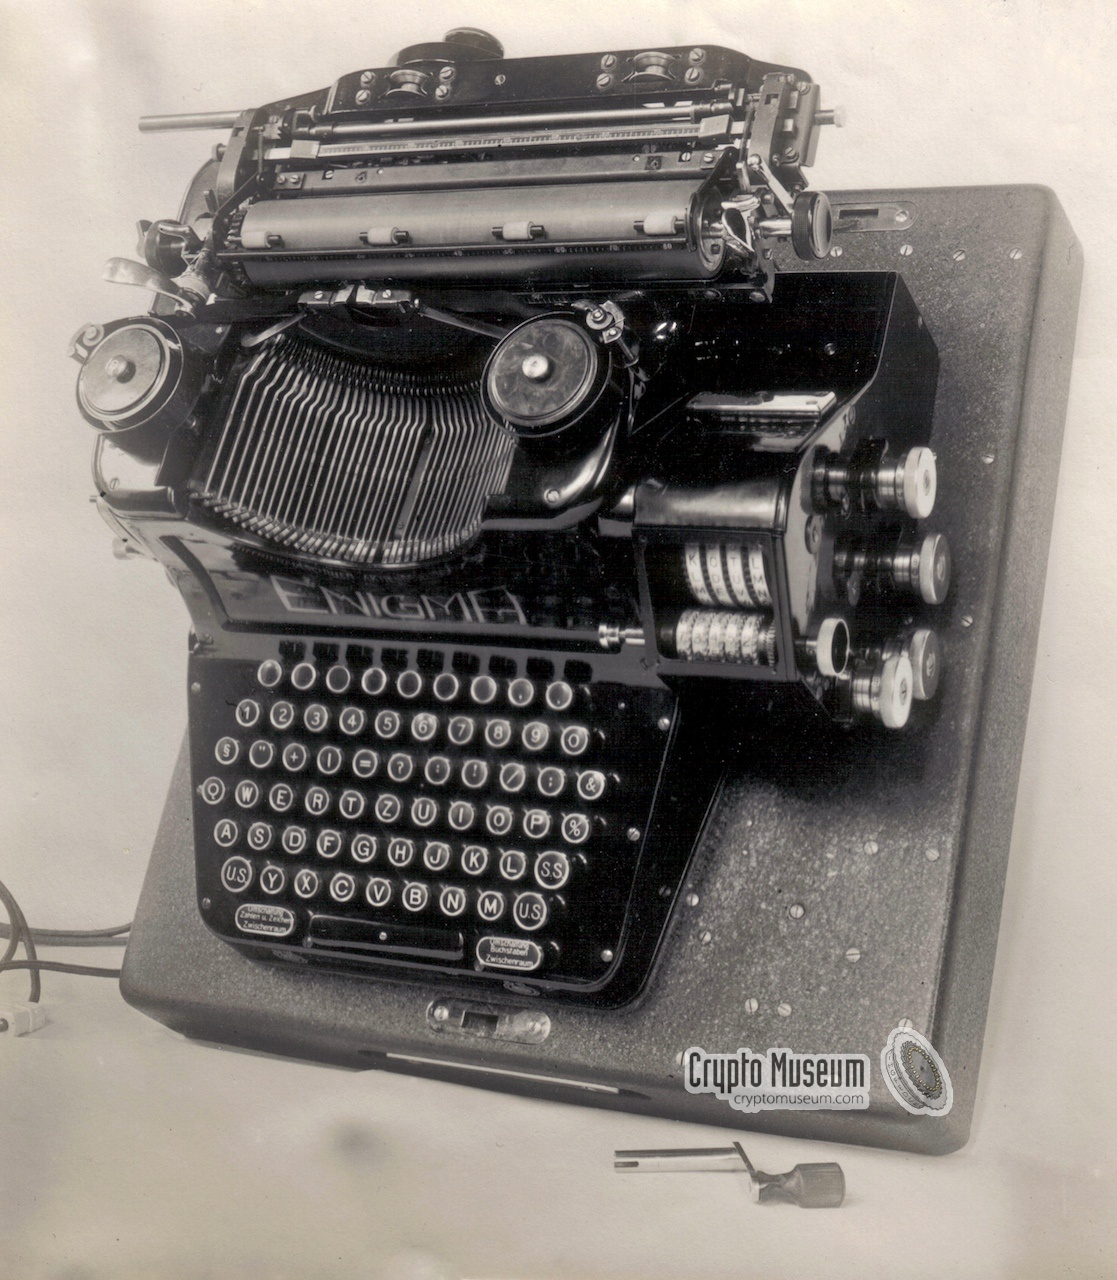
\includegraphics[scale=.1]{IMG/modelB.jpg}
\caption{\scriptsize Model D}
\end{figure}
\end{column}

\begin{column}{.5\textwidth}
\begin{figure}
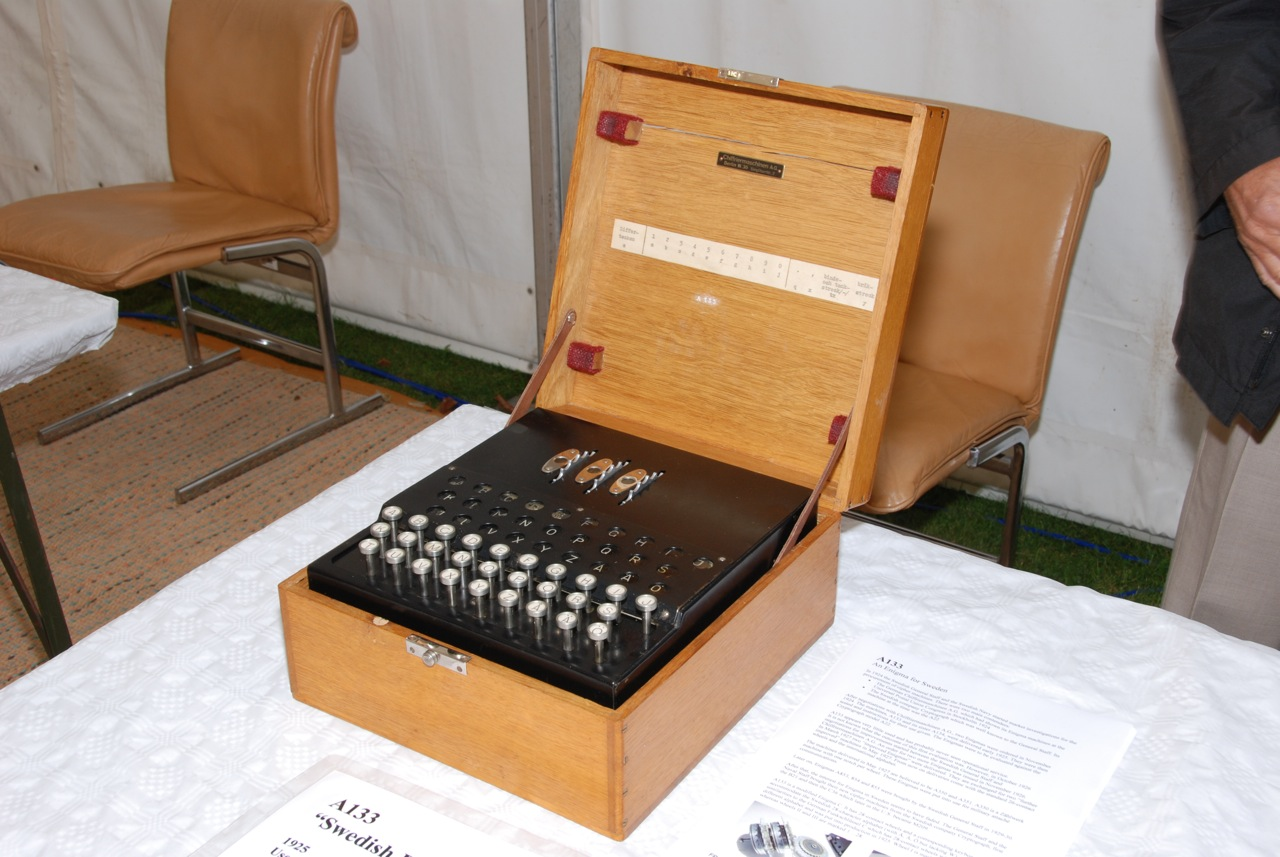
\includegraphics[scale=.5]{IMG/modelC.jpg}
\caption{\scriptsize Model C, with first light-up board}
\end{figure}
\end{column}
\end{columns}
\end{frame}


\begin{frame}
\frametitle{Portable Enigma}

Starting with model C, the Enigma was a portable device which looked similar to a typewriter.  

\begin{figure}
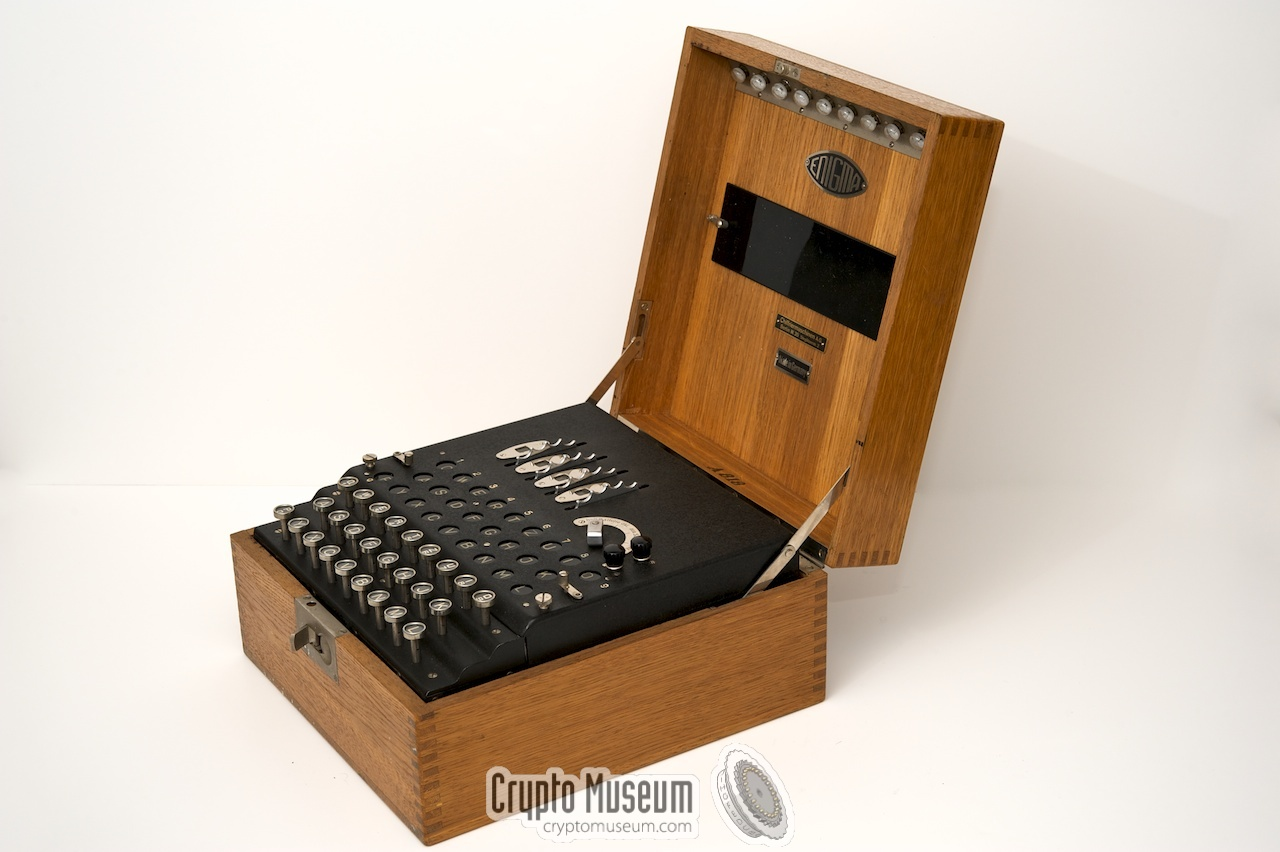
\includegraphics[scale=.1]{IMG/modelD.jpg}
\caption{\scriptsize Enigma Model D}
\end{figure}

Due to the Enigma Machine the German army had the strongest cryptographic cipher which existed at that point in time. 
\end{frame}


\section{Construction}

\begin{frame}
\frametitle{How Enigma Works}
\small 
To encrypt a message, starting with the first letter you press down on its key on the keyboard. Above the keyboard, a letter lights up which represents its ciphertext.\newline

\begin{center}
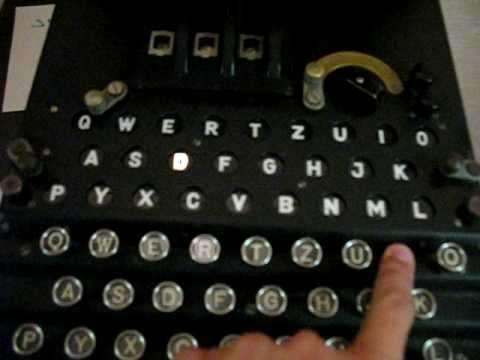
\includegraphics[scale=.2]{IMG/lamp}
\end{center}

This ciphertext was is out. It is decrypted using the same process, where typing in the ciphertext letter caused the plaintext letter to light up.\newline

Let's start by watching the following video on how the Enigma machine works:
\url{https://www.youtube.com/watch?v=ASfAPOiq_eQ}
\end{frame}


\begin{frame}
\frametitle{The Path}

\small
The electrical current sent out by typing in a letter originated at the keyboard and went through several steps: the \textbf{plugboard}, the \textbf{rotors}, the \textbf{reflector}, then back through the rotors and plugboard to the \textbf{lampboard}.

\begin{figure}
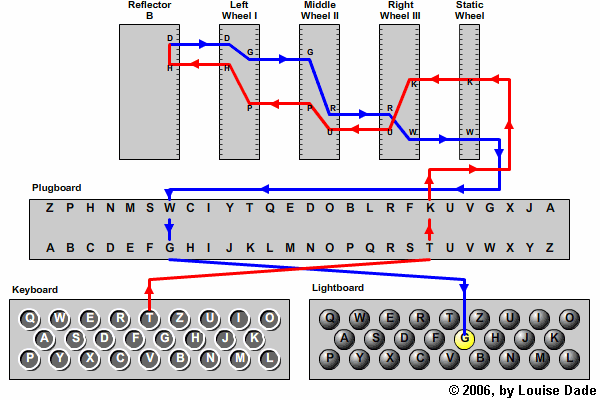
\includegraphics[scale=.45]{IMG/wiring}
\caption{\scriptsize Graphic from: \url{http://enigma.louisedade.co.uk/howitworks.html}}
\end{figure}
\end{frame}

\begin{frame}
\frametitle{Keyboard}

Pressing on the letter sends an electrical charge through the machine. 
\begin{center}
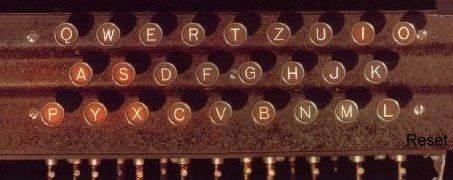
\includegraphics[scale=.5]{IMG/keyboard}
\end{center}
\end{frame}

\begin{frame}
\frametitle{Plugboard}

This signal first goes through the \textbf{plugboard}.
\begin{center}
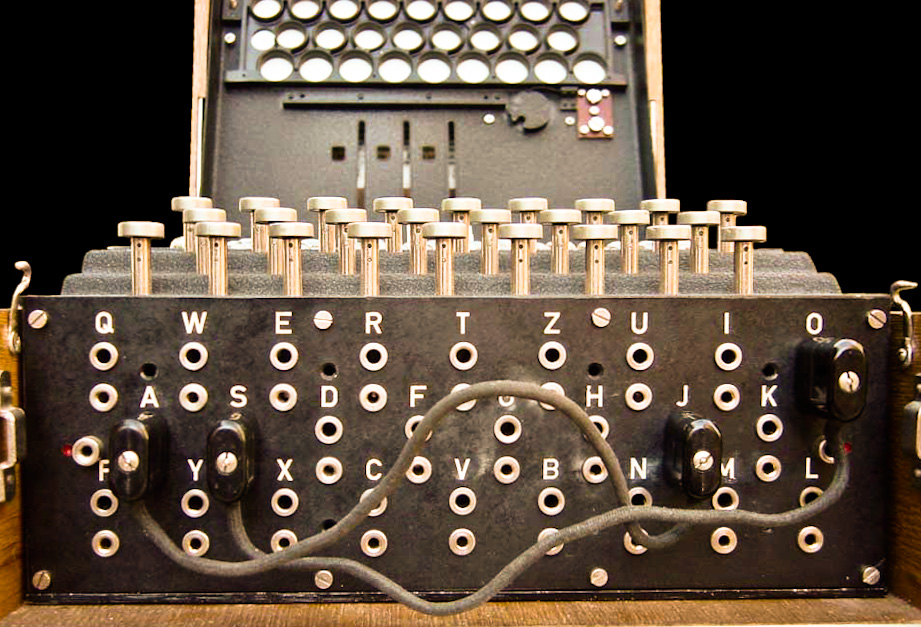
\includegraphics[scale=.7]{IMG/plugboard}
\end{center}
The plugboard uses \textbf{plugs} to wire up one letter to another, diverting its signal. If `A' is plugged in to `F', then the letter will now be interpreted by the machine as an `F'.
\end{frame}


\begin{frame}
\frametitle{Plugboard}

Later versions of the machine used 10 plugs to connect pairs of letters.
\begin{figure}
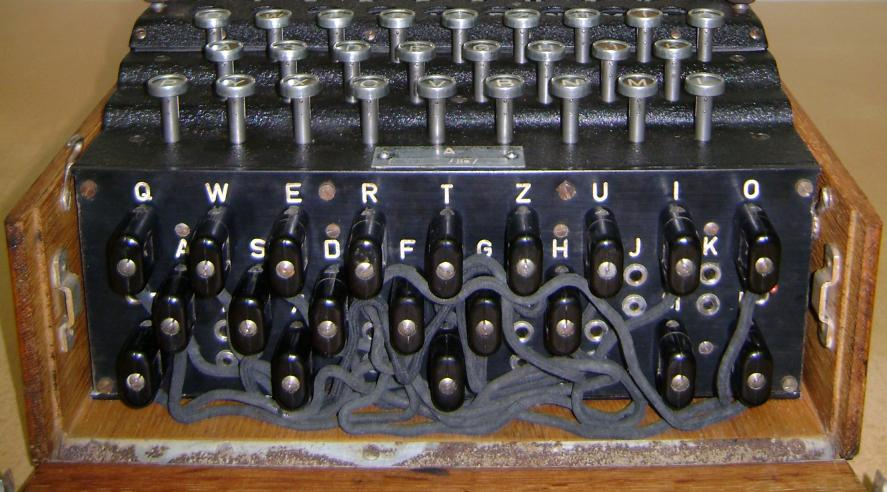
\includegraphics[scale=.2]{IMG/plugboard2}
\end{figure}

\textbf{How many ways were there to connect pairs of letters on the enigma machine?}
\end{frame}


\begin{frame}
\frametitle{Plugboard Combinations}

\textbf{How many ways were there to connect pairs of letters on the enigma machine?} \newline

There are $26 \choose 2$ ways of plugging in the first wire. For each of these combinations there are $24 \choose 2$ ways to plug in the second wire, and for each of those combinations there are $22 \choose 2$ ways to plug in the third wire, all the way down to $8\choose 2$ ways of plugging in the tenth wire. \newline

After multiplying this out, we must divide by $10!$, the number of ways to permute these wires -- since the order in which the pairs of wires are selected does not matter.
\end{frame}


\begin{frame}
\frametitle{Plugboard Combinations}

This yields a total of 
\[
\frac{{26 \choose 2 } {24 \choose 2 } {22 \choose 2 } {20 \choose 2 }{18 \choose 2 }{16 \choose 2 }{14 \choose 2 }{12 \choose 2 }{10 \choose 2 }{8 \choose 2 }}{10!}
\]
combinations, which works out to be 
\[
150,738,274,937,250.
\]
\end{frame}


\begin{frame}
\frametitle{Rotors}

\begin{columns}
\begin{column}{.6\textwidth}
\begin{figure}
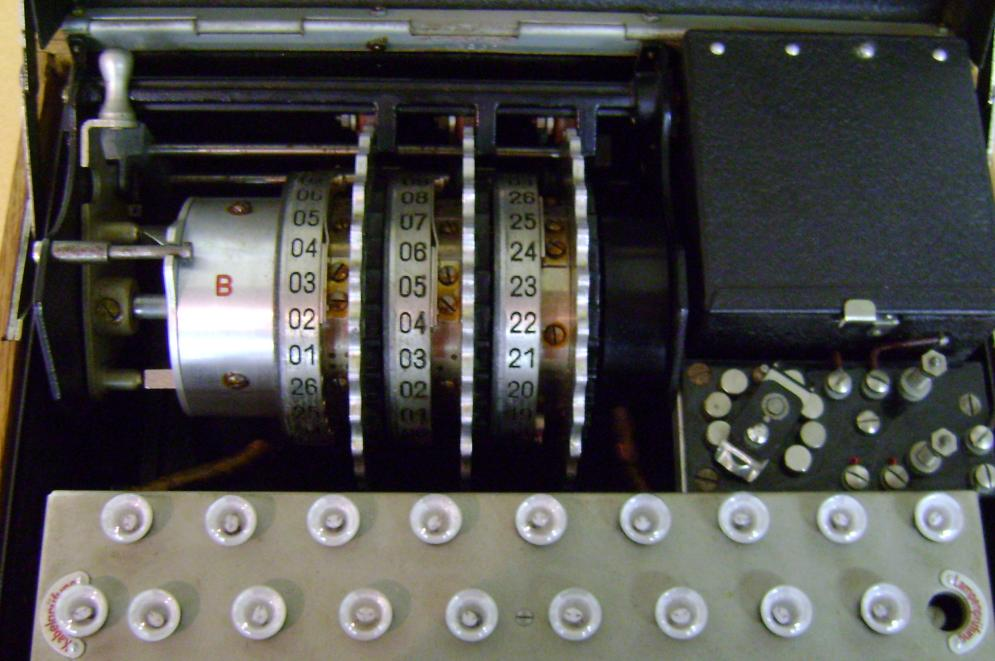
\includegraphics[scale=.18]{IMG/rotors}

\end{figure}
\end{column}
\begin{column}{.4\textwidth}
After going through the plugboard, the electrical charge is sent through three \textbf{rotors}. Each rotor permutes the letters, taking it in and outputting a different letter. The letter bounces off a reflector at the end, passes back through the rotors, and then the board lights up with the encrypted output. 
\end{column}
\end{columns}
\end{frame}


\begin{frame}
\frametitle{Inserting Rotors}

The rotors can be taken out of the machine. The machine has five rotors, and three of these are chosen to go into the three slots. \textbf{How many ways are there of positioning the five rotors in the three slots?}\newline

There are 
\[
5\times 4 \times 3 = 60
\]
ways of choosing the rotors' starting positions. 
\end{frame}


\begin{frame}
\frametitle{Rotor Movement}

The machine was designed so that the rotors would... rotate! After typing in the first letter, the first rotor ``clicks'' and rotates into a second position. It rotates through all 26 positions, then the second rotor ``clicks'', and after going through all positions on the second rotor the process repeats again with the third rotor. This leads to 
\[
26 \times 26 \times 26 = 17,576
\] 
possible combinations before encryptions begin to repeat! 
\end{frame}

\begin{frame}
\frametitle{Rotor Positions}

\textbf{How many possible starting positions are there for the rotors in the Enigma Machine?}\newline

We use the same calculation as on the previous slide. There are
\[
26 \times 26 \times 26 = 17,576
\] 
possible starting positions for the three rotors in the machine. 
\end{frame}

\begin{frame}
\frametitle{Reflector}
\begin{columns}
\begin{column}{.5\textwidth}
\begin{figure}
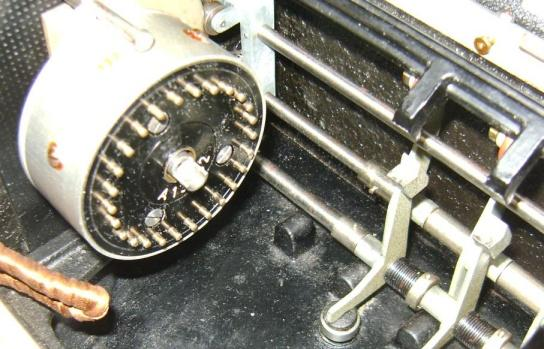
\includegraphics[scale=.25]{IMG/reflector}

\end{figure}
\end{column}
\begin{column}{.5\textwidth}
After going through the three rotors, the signal hits the ``reflector." There are two reflectors in the Enigma machine which are each set up differently -- most commonly used was the B reflector. They transform the letter to a different letter and send it back through the rotors in the reverse direction. 
\end{column}
\end{columns}
\end{frame}


\begin{frame}
\frametitle{Reverse Journey}

The reverse journey works the same way as the forward journey -- the signal is sent through the three rotors and permuted three times. \newline

After this the signal is reversed through the plugboard before being sent to the \textbf{lampboard}.
\end{frame}


\begin{frame}
\frametitle{The Lampboard}

The lampboard is the final stop for the electrical current -- it lights up the lamp for the letter of the ciphertext. 
\begin{figure}
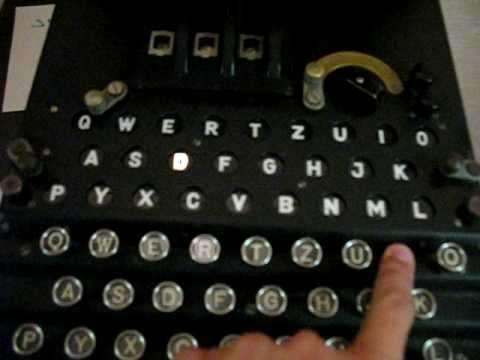
\includegraphics[scale=.35]{IMG/lamp}
\end{figure}
Because of the rotating rotors, you can press the same letter over and over but the letter which lights up changes each time. 
\end{frame}

\section{Bombe}

\begin{frame}
\frametitle{Breaking The Enigma}

\begin{columns}
\begin{column}{.5\textwidth}
\begin{figure}
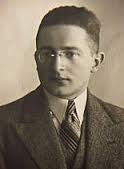
\includegraphics[scale=1]{IMG/rejewski}
\caption{\scriptsize Marian Rejewski}
\end{figure}
\end{column}
\begin{column}{.5\textwidth}\small
The first attempt at breaking the Enigma was led by Polish cryptanalysts Marian Rejewski, Henryk Zygalski and Jerzy Rozicki at the Polish cipher office \textbf{Biuro Szyfrow}. They created a machine called the \textbf{Bomba Machine}, which sped up the process of decrypting early Enigma Machine messages. This machine works completely differently from the Enigma. 
\end{column}
\end{columns}
\end{frame}

\begin{frame}
\frametitle{Bomba Machine: Exploiting A Weakness}

At first the Enigma Machine's key management system was incredibly vulnerable. At the beginning of each message, the randomly chosen message key was encrypted and sent twice. The Polish cryptographers used this in order to deduce the key each day. \newline

When the Germans realized this weakness, they stopped using this key distribution method. This increase in the sophistication of the enigma led to a necessity for a new cryptanalytic attack.
\end{frame}


\begin{frame}
\frametitle{Key Distribution: Code Books}

\begin{columns}
\begin{column}{.55\textwidth}
\begin{figure}
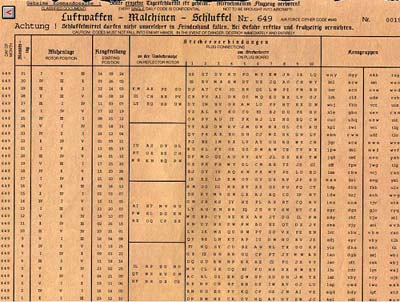
\includegraphics[scale=3.5]{IMG/keysheet}
\end{figure}
\end{column}
\begin{column}{.45\textwidth}
As this is a private key encryption system, the Germans needed a way of distributing private keys. At the beginning of each moth a \textbf{code book}/\textbf{keysheet} was given to the operators of the Enigma machines. This gave the key to be used each day, where the key consisted of rotor and plugboard settings. 
\end{column}
\end{columns}
\end{frame}

\begin{frame}
\frametitle{Bletchley Park}

\begin{columns}
\begin{column}{.6\textwidth}
\begin{figure}
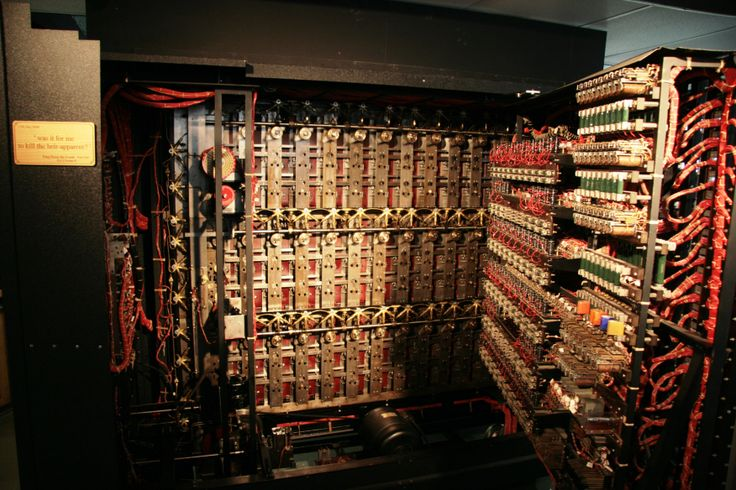
\includegraphics[scale=.25]{IMG/bombe}
\caption{\scriptsize The Bombe Machine}
\end{figure}
\end{column}
\begin{column}{.4\textwidth}
The Polish shared information on the mechanics of the Enigma machine with the British in 1939. Cryptographers at \textbf{Bletchley Park} designed the \textbf{Bombe Machine}, which weighs in at around 1 ton, to crack the Enigma.
\end{column}
\end{columns}
\end{frame}



\begin{frame}
\frametitle{Bombe Machine: Exploiting Another Weakness}

The key observation leading to the construction of the Bombe machine was that a letter was never encrypted as itself. Furthermore certain phrases were often included in messages, such as ``Wetterbericht'' (Weather Report) and ``Heil Hitler.'' Turing and Welchman designed the Bombe machine using these words along with the aforementioned observation. \newline

Let's watch the following video on how the cryptanalysts exploited this weakness (start at 34 seconds):
\url{https://www.youtube.com/watch?v=V4V2bpZlqx8}
\end{frame}


\begin{frame}
\frametitle{Alan Turing}

\begin{columns}
\begin{column}{.5\textwidth}
\begin{figure}
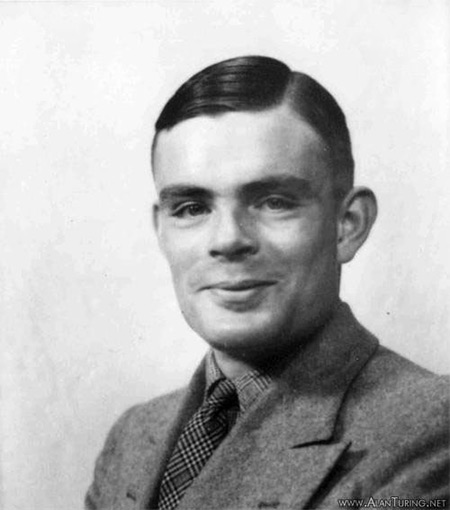
\includegraphics[scale=.3]{IMG/turing}
\caption{\scriptsize Alan Turing}
\end{figure}
\end{column}
\begin{column}{.5\textwidth}
Alan Turing was one of the main forces behind the design of the British Bombe machine. He was recently popularized in the film \textbf{The Imitation Game}. \newline

He is known as 	``the father of computer science'' and is responsible for designing the \textbf{Turing machine}, a mathematical model for computing still used today, as well as the \textbf{Turing test}, a test for artificial intelligence.
\end{column}
\end{columns}
\end{frame}

\begin{frame}
\frametitle{Other Cryptographers at Bletchley}
\small
There were many other people on the team at Bletchley Park. \textbf{Gordon Welchman} designed an enhancement to Turing's machine which significantly increased its speed. \textbf{Joan Clarke} also played an instrumental role at Bletchley Park -- although sexism meant she was paid less and prevented from progressing as far in her career.

\begin{columns}
\begin{column}{.5\textwidth}
\begin{figure}
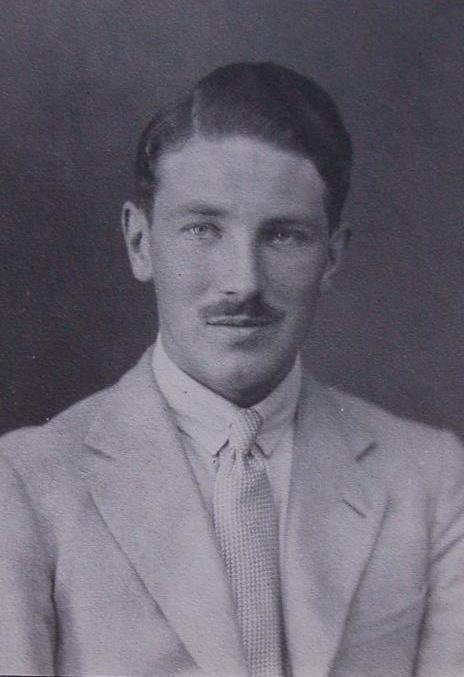
\includegraphics[scale=.2]{IMG/welchman}
\end{figure}
\end{column}
\begin{column}{.5\textwidth}
\begin{figure}
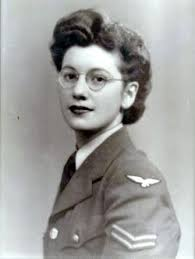
\includegraphics[scale=.5]{IMG/clarke}
\end{figure}
\end{column}
\end{columns}
\end{frame}

\begin{frame}
\frametitle{Turing's Death and Legacy}

In 1952 Alan Turing was convicted of ``gross indecency'' after acknowledging that he was a homosexual to the cops while reporting a robbery. \newline

Turing was stripped of his security clearance and banned from consulting with the GCHQ (British intelligence). He was given the choice between chemical castration and prison. He committed suicide in 1954.\newline

In August 2014 the queen posthumously pardoned Alan Turing. In September 2016 this pardon was expanded posthumously to cover all other men convicted of indecency offenses for homosexuality throughout history. This law is known informally as the \textbf{Alan Turing Law}.
\end{frame}

\begin{frame}
\frametitle{References}

\begin{itemize}
\item Counting plugboard settings: \url{http://www.codesandciphers.co.uk/enigma/steckercount.htm}
\item How the machine works: \url{http://enigma.louisedade.co.uk/howitworks.html}
\item History \& How it works: \url{https://www.theguardian.com/technology/2014/nov/14/how-did-enigma-machine-work-imitation-game}
\item History: \url{http://cs-exhibitions.uni-klu.ac.at/index.php?id=282}
\item History: \url{https://plus.maths.org/content/exploring-enigma}
\end{itemize}
\end{frame}
\end{document}


